\chapter{Conceptos de autonomía}

\begin{enpocas}
El ciclo percibir--decidir--actuar, las máquinas de estados, cómo se planea recorrer toda una zona,
cuándo vale la pena volver a mirar, qué es el GPS y cómo se pasa de metros a latitud y longitud, y qué
es un LiDAR.
\end{enpocas}

\section{Percibir, decidir, actuar}

Un dron autónomo repite sin parar tres pasos. \emph{Percibir}: la cámara, el detector y el localizador
le dicen dónde podría haber personas. \emph{Decidir}: la misión elige a dónde ir (seguir la franja,
volver a mirar una candidata dudosa, aterrizar). \emph{Actuar}: manda la consigna a PX4 o ArduPilot, que
mueven los motores.

\section{Máquinas de estados}

La misión se organiza en \textbf{estados}: despegue, barrido, re-observación, aterrizaje y fin. En cada
uno hace una cosa y cambia de estado cuando se cumple una condición (``llegué a 30~m'', ``terminé la
última franja''). Es fácil de entender, de probar y de registrar: el JSON de cada vuelo trae la lista de
cambios de estado con su hora.

\begin{ejemplo}
Una lavadora: llenar, lavar, enjuagar, centrifugar. Cada etapa termina por tiempo o por un sensor, y
pasa a la siguiente.
\end{ejemplo}

\section{Cubrir toda la zona}

Si no se sabe dónde está la persona hay que mirar todo: \textbf{planificación de cobertura}. Lo clásico
es ir y venir en franjas paralelas, como al podar un jardín. La clave es la separación: con la cámara
hacia abajo a 30~m, la huella mide $71\times53$~m; con franjas separadas 42~m (60~\% de la huella) cada
punto se ve al menos dos veces y queda margen para el viento.

\begin{figure}[H]
\centering
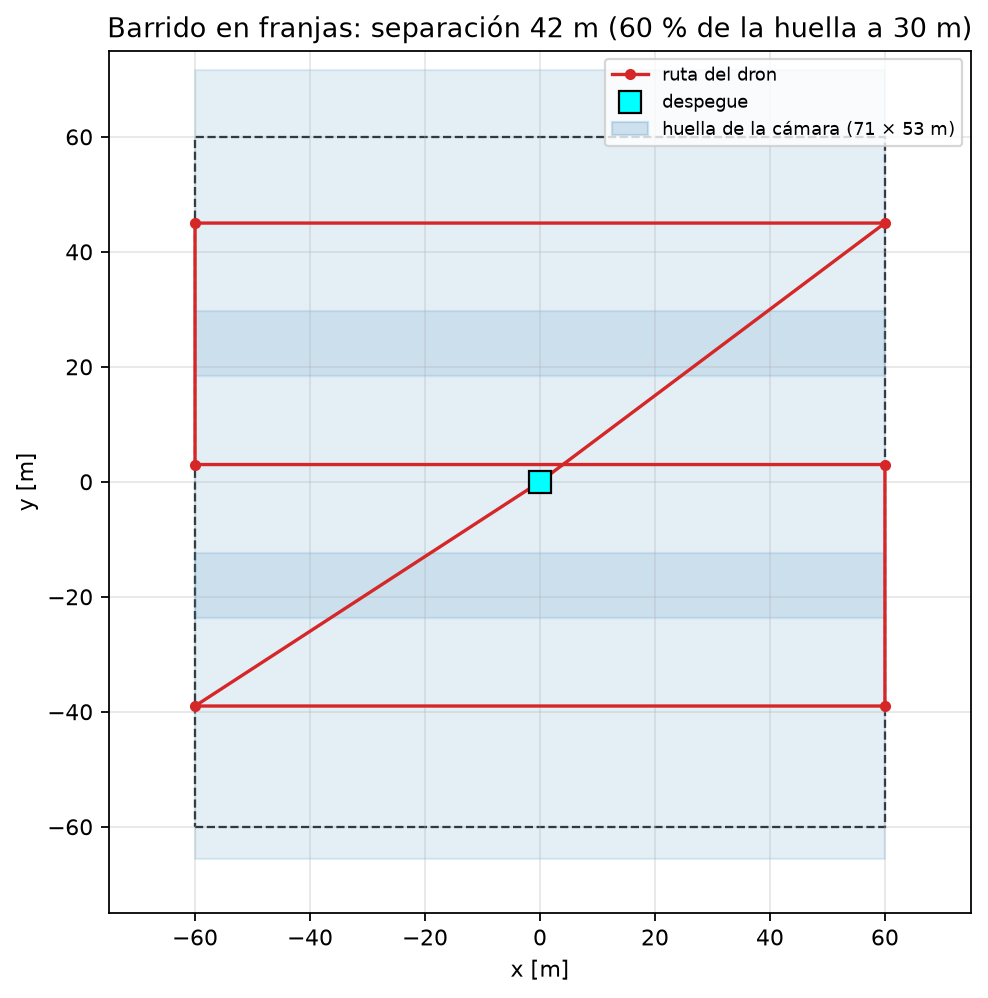
\includegraphics[width=0.65\textwidth]{franjas.png}
\caption{El barrido del proyecto: tres franjas cubren el cuadrado de 120~m con traslape.}
\end{figure}

\section{Volver a mirar: el valor de la información}

Una candidata con confianza intermedia (por ejemplo entre 0.3 y 0.6) es dudosa: puede ser una persona
tapada o una sombra. Bajar a verla desde otro ángulo cuesta tiempo y batería, pero puede convertir una
duda en una persona encontrada (o descartar una falsa alarma). Esa es la estrategia de
\textbf{re-observación}: ¿compensa? Responder esa pregunta con datos es el objetivo de la campaña
experimental (capítulo~\ref{cap:experimental}).

\section{GPS: de metros a latitud y longitud}

La simulación trabaja en metros sobre un plano (ENU); los rescatistas necesitan \textbf{coordenadas GPS}.
La Tierra se modela como un elipsoide (\textbf{WGS84}). La conversión exacta pasa el punto del plano
local a coordenadas cartesianas centradas en la Tierra (ECEF) y de ahí a latitud, longitud y altitud
(\cod{mision/geo.py}).

\begin{figure}[H]
\centering
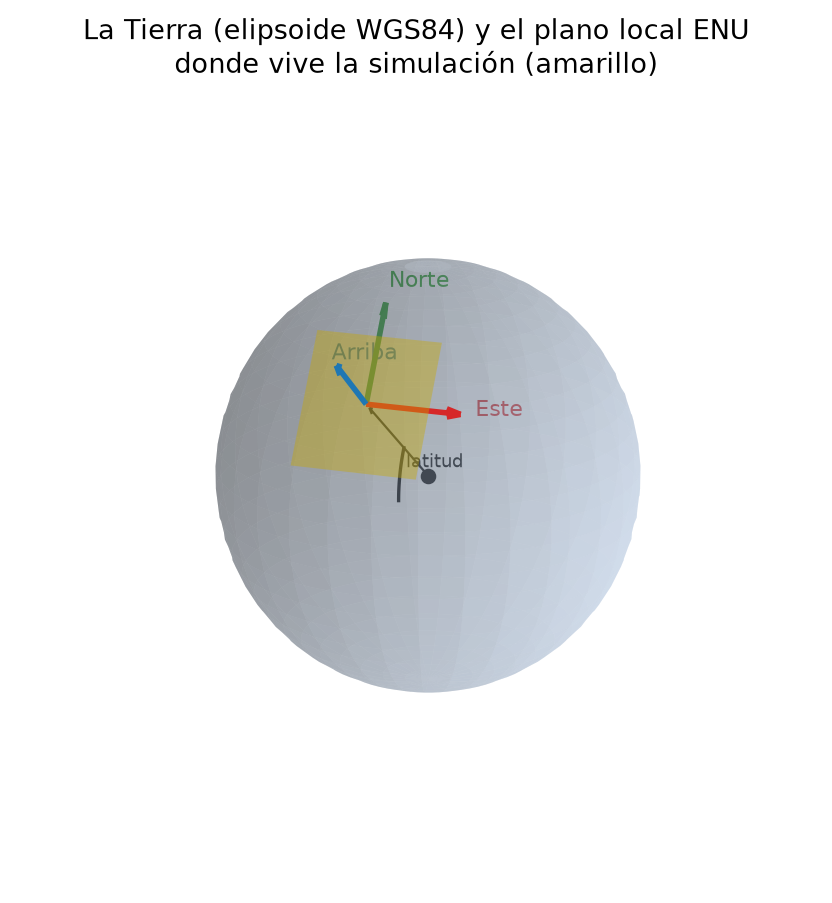
\includegraphics[width=0.55\textwidth]{c_tierra.png}
\caption{El plano local ENU de la simulación es tangente a la Tierra en el origen del mundo.}
\end{figure}

\begin{tecnico}
A 19.5° de latitud, un grado de latitud mide unos 110.8~km y uno de longitud unos 105~km: seis
decimales en las coordenadas equivalen a $\approx$10~cm.
\end{tecnico}

\section{LiDAR}

Un \textbf{LiDAR} mide la distancia al primer obstáculo en muchas direcciones lanzando pulsos láser. Da
una nube de puntos: no sabe \emph{qué} es cada punto, pero sí dónde está. La cámara reconoce personas;
el LiDAR evita chocar.

\begin{figure}[H]
\centering
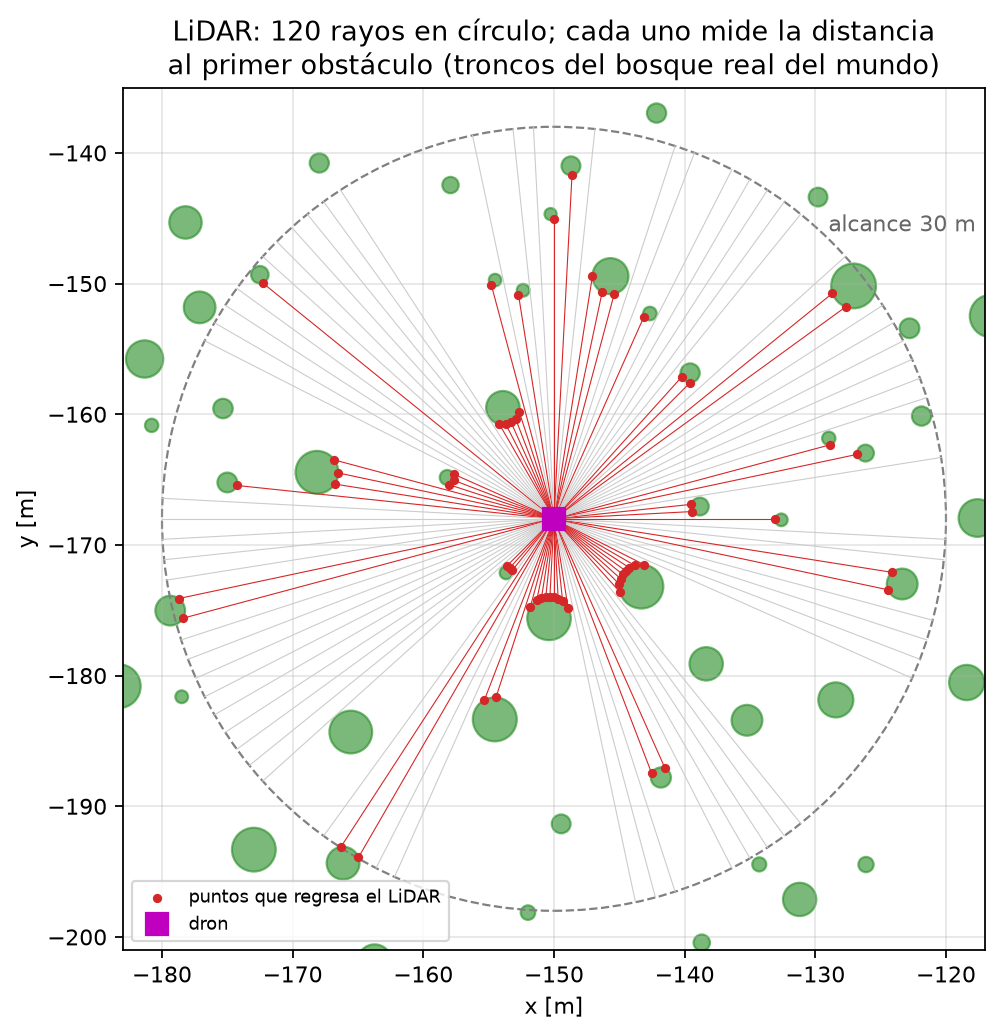
\includegraphics[width=0.55\textwidth]{c_lidar.png}
\caption{Una capa de un LiDAR en un bosque: cada rayo rojo toca un tronco.}
\end{figure}

La evasión del proyecto es reactiva, del tipo VFH: divide las direcciones alrededor del dron en 72
sectores, marca los bloqueados por obstáculos cercanos y toma el sector libre más parecido a la
dirección deseada.

\begin{figure}[H]
\centering
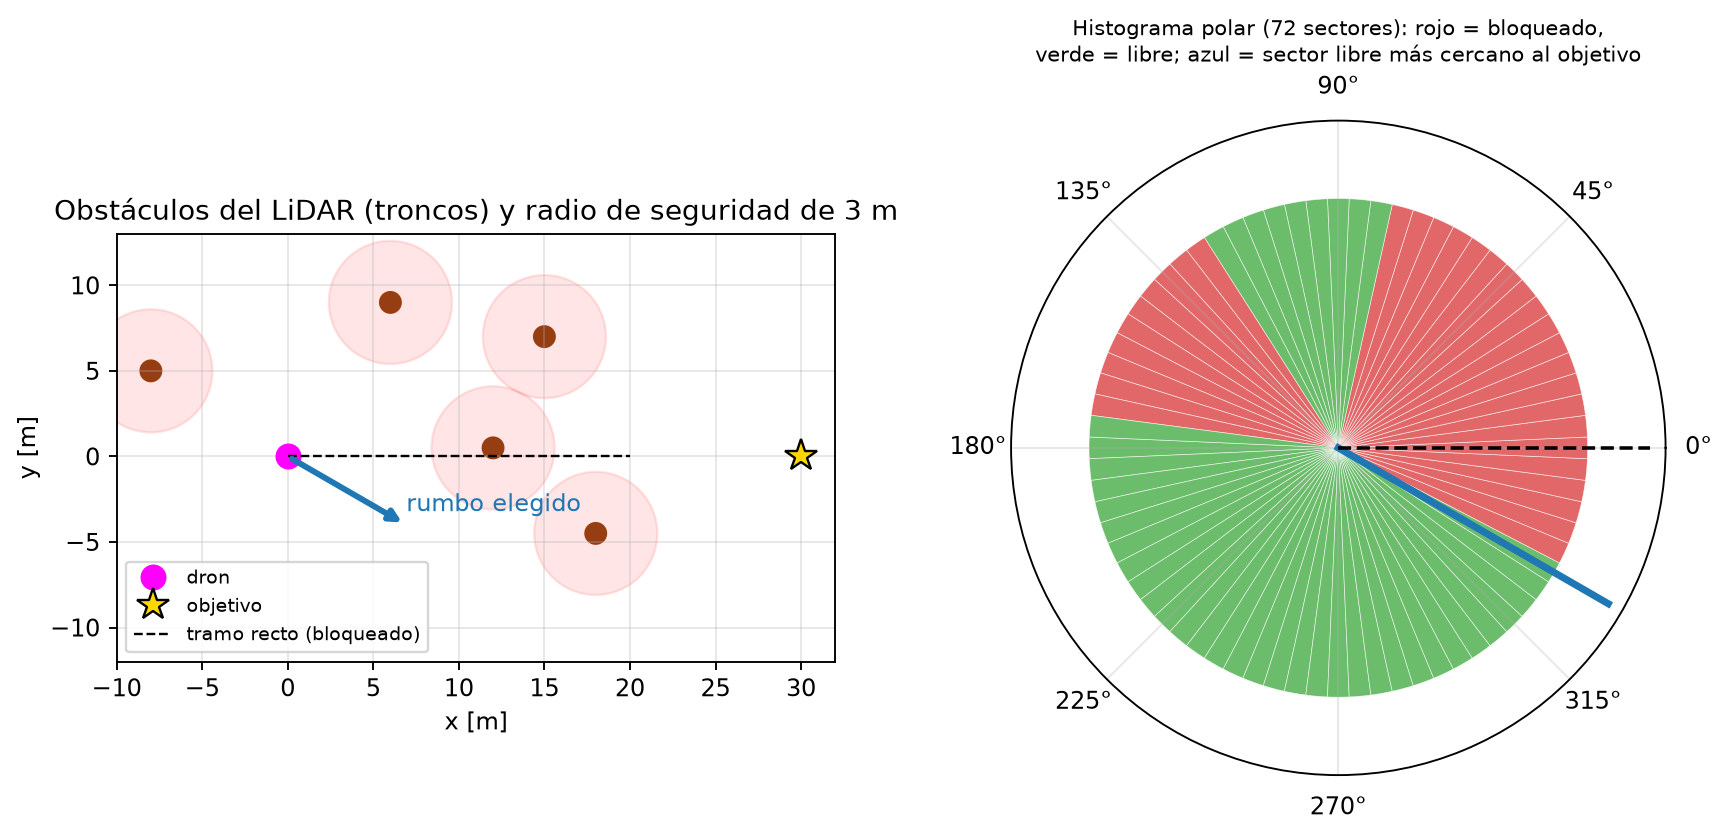
\includegraphics[width=\textwidth]{vfh.png}
\caption{Evasión con histograma polar.}
\end{figure}
